\PassOptionsToPackage{subsection=false}{beamerouterthememiniframes}
\documentclass[9pt,compress,t,aspectratio=169]{beamer}
\usetheme[
	bullet=circle,
	alternativetitlepage=true,
	titleline=true,
	titlepagelogo=img/loghi_insieme,
]{mathlab}
\usepackage[utf8]{inputenc}
\usepackage[T1]{fontenc}
\usepackage[english]{babel}
\usepackage{amsmath}
\usepackage{amsthm}
\usepackage{amsfonts}
\usepackage{graphicx}
\usepackage{caption}
\usepackage{subcaption}
\usepackage{verbatim} % per comment
\usepackage{lmodern} % font più chiaro
\usepackage{ragged2e}
\usepackage{bm}
\usepackage{tikz}
\usepackage[thicklines]{cancel}
\usepackage{xcolor}
\usepackage{wasysym}
\usepackage{units}
\usepackage{tikzsymbols}
\usepackage{multimedia}
\usepackage{graphicx}
\usepackage{pgfplots}
\usepackage{pgfplotstable}
\usepackage{media9}


\newcommand\Ccancel[2][black]{\renewcommand\CancelColor{\color{#1}}\cancel{#2}}
\newcommand{\cfbox}[2]{%
    \colorlet{currentcolor}{.}%
    {\color{#1}%
    \fbox{\color{currentcolor}#2}}%
}


\newcommand{\bad}{\Sadey[2][red]}
\newcommand{\good}{\Smiley[2][green]}

\newcommand{\one}{$[1]$}
\newcommand{\two}{$[2]$}
\newcommand{\three}{$[3]$}
\newcommand{\scpr}[2]{\left(#1,#2\right)_\Omega}
\newcommand{\scprb}[2]{\sum_b \left(#1,#2\right)_{\partial\Omega \cap \Gamma_b }}
\newcommand{\scpre}[2]{\sum_e\left(#1,#2\right)_{\Omega_e}}


\setbeamertemplate{navigation symbols}{}


\usepackage{tikz}
\usepackage{tikzsymbols}
\usetikzlibrary{shadows}

\usetikzlibrary{decorations.pathreplacing,calligraphy}


\graphicspath{%
	{figures/}%
}

% Norma
\newcommand\norm[1]{\left\lVert#1\right\rVert}

%---------------> Text style
\newcommand{\Tr}{\mathrm{T}}
\newcommand{\diag}{\mathop{\mathrm{diag}}}
\newcommand{\xx}{\boldsymbol{x}}
\newcommand{\dV}{\,\mathrm{d}\Omega}
\newcommand{\dS}{\,\mathrm{d}\partial\Omega}
\newcommand{\vecn}{\boldsymbol{\mathbf n}}
\newcommand{\Ndofe}{N^e_\mathrm{dof}}
\newcommand{\Ndim}{{N_\mathrm{dim}}}
\newcommand{\Neqn}{{N_\mathrm{eq}}}
\newcommand{\E}{\mathrm{E}}
\newcommand{\FF}{\boldsymbol{\mathsf{R}}} 
\newcommand{\JJ}{\mathbb{J}} 
\newcommand{\bbf}{{\mathbf {f}}}
\newcommand{\bxx}{{\mathbf {x}}}
\newcommand{\bn}{{\mathbf {n}}}
\newcommand{\n}{{\mathbf {n}}}
\newcommand{\s}{\sqrt{2}}
\newcommand{\is}{\frac{\sqrt{2}}{2}}
\newcommand{\hf}{\hat{f}}

\newcommand{\dpar}[2]{\dfrac{\partial #1}{\partial #2}}
\newcommand{\bu}{\mathbf{u}}
\newcommand{\ub}{\mathbf{u}}
\newcommand{\bv}{\mathbf{v}}
\newcommand{\Bv}{\underline{\mathbf{v}}}
\newcommand{\bbv}{\mathbf{v}}
\newcommand{\Bbv}{\underline{\mathbf{v}}}
\newcommand{\bF}{\mathbf{F}}
\newcommand{\bG}{\mathbf{G}}
\newcommand{\bbS}{\mathbf{S}}
\newcommand{\bFF}{\mathcal{F}}
\newcommand{\bbF}{\mathbf{\mathcal{F}}}
\newcommand{\bK}{\mathbf{K}}
\newcommand{\bbu}{\mathbf{u}}
\newcommand{\bbg}{\mathbf{g}}
\newcommand{\hbbg}{\hat{\mathbf{g}}}
\newcommand{\hbbf}{\hat{\mathbf{f}}}
\newcommand{\hbbU}{\hat{\mathbf{U}}}
\newcommand{\hbbfe}{\hat{\mathbf{f}}_{\sigma,\sigma'}}
\newcommand{\ba}{\mathbf{a}}
\newcommand{\bx}{\mathbf{x}}
\newcommand{\x}{\mathbf{x}}
\newcommand{\by}{\mathbf{y}}
\newcommand{\red}[1]{\textcolor{red}{#1}}
\newcommand{\blue}[1]{\textcolor{blue}{#1}}
\newcommand{\magenta}[1]{\textcolor{magenta}{#1}}
\newcommand{\ICI}{\red{\large{ICI}}}

% ---- Notation Philipp
\newcommand{\ww}[1]{\underline{#1}}
\renewcommand{\div}{\operatorname{div}}
\newcommand{\est}[1]{\left\langle#1\right\rangle}
\newcommand{\bU}{\mathbf{U}}
\newcommand{\bH}{\mathbf{H}}
\newcommand{\dd}{\mathrm{d}}
\newcommand{\bV}{\mathbf{V}}
\newcommand{\mean}[1]{\overline{#1}}
\newcommand{\bbfh}{{\mathbf {f}^h}}
\newcommand{\Ol}{\mathcal{O}}
\newcommand{\WW}{\mathrm{W}}
\newcommand{\LL}{\mathcal{L}}
\newcommand{\II}{\hat{I}_0}
\newcommand{\1}{\begin{pmatrix}
		1\\
		1
\end{pmatrix}}
\newcommand{\e}[1]{\mathrm{e^{#1}}}
\newcommand{\VV}{\mathcal{V}}

\newcommand{\CU}{\mathcal{U}}

\newcommand{\NDG}{N_h}
\newcommand{\NRB}{N_{RB}}
\newcommand{\zRB}{z_{RB}}
\newcommand{\zDG}{z_h}
\newcommand{\VDG}{V_h}
\newcommand{\VRB}{V_{RB}}
\newcommand{\Naff}{N_{affine}}

%%%%%Dante 
\newcommand{\diff}[1]{{\mathrm{d}{#1}}}
\newcommand{\dotprod}{\boldsymbol \cdot}
\newcommand{\ddt}[1]   {\frac{\partial{#1}}{\partial{t}}}
\newcommand{\ddx}[1]   {\frac{\partial{#1}}{\partial{x}}}
\newcommand{\ddy}[1]   {\frac{\partial{#1}}{\partial{y}}}
\newcommand{\dsddt}[1] {\dfrac{\partial{#1}}{\partial{t}}}
\newcommand{\txddt}[1] {\tfrac{\partial{#1}}{\partial{t}}}
\newcommand{\ddp}[2]   { \frac{\partial #1}{\partial #2}}
\newcommand{\dsddp}[2] {\dfrac{\partial #1}{\partial #2}}
\newcommand{\txddp}[2] {\tfrac{\partial #1}{\partial #2}}
\newcommand{\ddo}[2]   { \frac{\diff #1}{\diff #2}}
\newcommand{\dsdo}[2]  {\dfrac{\diff #1}{\diff #2}}
\newcommand{\txddo}[2] {\tfrac{\diff #1}{\diff #2}}
\newcommand{\Div}[1] { \boldsymbol{\nabla} \!\dotprod #1 }
\newcommand{\Grad}[1] { \boldsymbol{\nabla} #1 }
\newcommand{\Gradr}[1]{\widetilde{\boldsymbol{\nabla} {#1}}}
\newcommand{\vect}[1] {\ww{#1}}
\newcommand{\versor}[1] {\hat{ \boldsymbol{#1}}}
\newcommand{\vzero}{\boldsymbol{0}}
\newcommand{\IdxM} {\mathbb{I}}
%----------------> Euler and NS equation
\newcommand{\vel}{\boldsymbol{v}}
\newcommand{\mm}{\boldsymbol{m}}
%\newcommand{\ee}{e}
\newcommand{\hh}{h}
\newcommand{\Et}{E^t}
\newcommand{\et}{e^t}
\newcommand{\Rgas}{\mathcal{R}}
\newcommand{\vecu}{\mathsf{u}}
\newcommand{\vecf}{\boldsymbol{\mathsf{f}}}
\newcommand{\vecfa}{\boldsymbol{\mathsf{f}}^a}
\newcommand{\vecfv}{\boldsymbol{\mathsf{f}}^v}
\newcommand{\Jac}{\boldsymbol{\mathsf{A}}}   
\newcommand{\viscT}{\mathbb{S}}
\newcommand{\Kgas}{\kappa}
%Numerical schemes
\newcommand{\xip}{x_{i+1/2}}
\newcommand{\xin}{x_{i-1/2}}

\newcommand{\yjp}{y_{j+1/2}}
\newcommand{\yjn}{y_{j-1/2}}

\newcommand{\iip}{i+1/2}
\newcommand{\iin}{i-1/2}

\newcommand{\jjp}{j+1/2}
\newcommand{\jjn}{j-1/2}

\newcommand{\Resjr}{\Phi^{j+\frac{1}{2}}_j}
\newcommand{\Resjl}{\Phi^{j-\frac{1}{2}}_j}

\newcommand{\Resjrn}{\Phi^{j+\frac{1}{2},n}_j}
\newcommand{\Resjln}{\Phi^{j-\frac{1}{2},n}_j}


\newcommand{\cc}[1]{\chi_{[t^0,t^{#1}]}}

\newcommand{\qq}{\hat{q}}

\newcommand{\tq}{\tilde{\mathrm{q}}}

\newcommand{\tqi}{\tilde{\mathrm{q}}_j^{i}}

\newcommand{\bs}{\mathrm{s}}
%\newcommand{\L}{\mathcal{L}}
\newcommand{\bS}{\mathcal{S}}

\renewcommand{\vec}[1]{\ww{#1}}
\newcommand{\mat}[1]{\underline{\underline{#1}}}



\usepackage{bbm}
\def\L{\mathcal{L}}
\def\I{\mathcal{I}}
\def\R{\mathbb{R}}
\def\bbc{\underline{\boldsymbol{c}}}
\def\bc{\boldsymbol{c}}
\def\br{\boldsymbol{r}}
\def\bd{\mathbf{d}}
\def\bbd{\underline{\mathbf{d}}}
\def\bphi{\underline{\phi}}
\def\M{\underline{\underline{\mathrm{M}}}}
\newcommand{\mass}{\mathbb M}

\newcommand{\Prod}{p}
\newcommand{\dest}{d}
\newcommand{\Ip}{\mathcal{I}}
\newcommand{\bby}{\mathbf{y}}

%colors



% Evidenziato
\newcommand{\TODO}[1]{{\color{red}#1}}
\newcommand{\highlight}[1]{\textbf{\color{bluemathlab}#1}}
\newcommand{\highlightB}[1]{\textbf{\color{black!15!orangemathlab}#1}}
\newcommand{\mathhighlight}[1]{\color{bluemathlab}#1}
\newcommand{\mathhighlightB}[1]{\color{black!15!orangemathlab}#1}

% Framebreaks: move continuation count from subtitle to title
\setbeamertemplate{frametitle continuation}[from second][]
\makeatletter 
\long\def\beamer@@frametitle[#1]#2{% 
	\beamer@ifempty{#2}{}{% 
		\gdef\insertframetitle{#2\ifnum\beamer@autobreakcount>1\relax{}\space(\insertcontinuationcountroman)\fi}% 
		\gdef\beamer@frametitle{#2}% 
		\gdef\beamer@shortframetitle{#1}% 
	}% 
}
\makeatother 

\setbeamercolor{blockcolor1}{fg=black,bg=bluemathlab!10}
\setbeamercolor{blockcolor2}{fg=black,bg=orangemathlab!10} 

\AtBeginSection[]
{{
		\setbeamertemplate{footline}[decolines theme without pages]
		\addtocounter{framenumber}{0}
		\begin{frame}
			\frametitle{Table of contents}
			\tableofcontents[currentsection]
		\end{frame}
}}

\title[MOR for Friedrichs' systems]{\LARGE \bf Reduced Order Models on a Variational Multi-Scale Model of Navier–Stokes: \\ 
foucs on wall law functions for boundary layer treatment\\
preliminary study}
\author[D. Torlo]{\Large\vspace{-1cm}\\\textbf{Davide Torlo, Giovanni Stabile,\\ Samuele Rubino, Gianluigi Rozza}} 
\institute[SISSA mathLab]{%
\vspace{-3mm}\\%
\small MathLab, Mathematics Area, SISSA International School for Advanced Studies, Trieste, Italy\\
\href{https://www.davidetorlo.it}{\underline{davidetorlo.it}}
}
\date{\vspace{-3mm}\\ CFC - Cannes - 26th April 2023\\
}


\begin{document}

%%%%%%%%%%%%%%%%%%%%%%
\begin{frame}[t,plain]
\addtocounter{framenumber}{-1}
\titlepage
\end{frame}


\begin{frame}{Motivation}
	\begin{minipage}{0.49\textwidth}
		\begin{block}{Fluid Simulations}
			\begin{itemize}
				\item Which \highlight{scale} can we approximate?
				\item Computational \highlightB{costs} vs \highlightB{accuracy}
				\item Large Eddy Simulations (LES)
				\item Variational Multi-Scale (\highlight{VMS})
				\item Weak Boundary conditions and \highlight{Wall-Law} for boundary layers to improve accuracy
				\item Turbolence 
			\end{itemize}
		\end{block}
	\end{minipage}\hfill
	\begin{minipage}{0.49\textwidth}
	\begin{block}{Model order reduction}
		\begin{itemize}
		\item \highlightB{Parametric} context or time prediction
		\item Further reduce costs
		\item \highlightB{Reduce} the computational cost for a new parameter/time
		\item Good approximation
		\item Challenges:
		\begin{itemize}
			\item Representability (turbolence, moving discontinuities)
			\item Stability			
		\end{itemize}
		\end{itemize}
	\end{block}
\end{minipage}\\
\begin{center}
	\visible<2->{
		\begin{minipage}{0.32\textwidth}
	\begin{block}{In this talk}
				\begin{itemize}
			\item Wall Law model
			\item \highlightB{POD-Galerkin} vs \highlightB{POD-NN}
			\item Flow past cylinder
				\end{itemize}
			\end{block}	
		\end{minipage}}\hspace{2mm}
	\visible<3->{
	\begin{minipage}{0.31\textwidth}
		\begin{block}{Not in this talk}
	\begin{itemize}
		\item Not (really) turbolent
		\item No special techniques for advection dominated structures
	\end{itemize} 
\end{block}	
\end{minipage}\hspace{2mm}}
\visible<4->{
\begin{minipage}{0.31\textwidth}
	\begin{block}{In the future}
\begin{itemize}
	\item VMS-Smagorinskij model % with LPS stabilization
	\item Hyper-reduction
	\item NN for wall laws
\end{itemize} 
\end{block}	
\end{minipage}
}

\end{center}


\end{frame}

\begin{frame}{Table of contents}
	\tableofcontents
\end{frame}

%
%\begin{frame}
%	\includemedia[
%	width=0.6\linewidth,
%	height=0.3\linewidth,
%	activate=pageopen,
%	addresource=figures/trial.avi,
%	flashvars={source=figures/trial.avi
%			&loop=true 
%			&autoPlay=true }
%	]{}{VPlayer.swf}
%\end{frame}
%%%%%%%%%%%%%%%%%%%%%%
\section{Indroduction to Variational Multi-Scale (VMS) model}

\begin{frame}{Navier--Stokes VMS\footnote{Y. Bazilevs, T.J.R. Hughes / Computers \& Fluids 36 (2007) 12--26}}
\begin{minipage}{0.49\textwidth}
	\only<1-3>{
	\visible<1-3>{
	\begin{block}{Navier--Stokes equations (strong)}
		\begin{equation*}
			\begin{cases}
					\frac{\partial \vec{u}}{\partial t} + (\vec{u} \cdot \nabla) \vec{u} + \nabla p - 2\div(\nu \nabla^s\vec{u})=0\\
									\nabla \cdot \vec{u} = 0\\
				\text{B.C. and I.C.}
			\end{cases}
		\end{equation*}
	\end{block}}
\visible<2-3>{
\begin{block}{Weak formulation}
\begin{align*}
	\begin{cases}
	&\scpr{\vec{v}}{\frac{\partial \vec{u}}{\partial t}} -\scpr{\nabla \vec{v}}{\vec{u}\otimes \vec{u}} + \scpr{q}{\nabla \cdot \vec{u}} - \\
	& \scpr{\nabla \cdot \vec{v}}{p} + \scpr{\nabla^s \vec{v}}{2\nu \nabla^s \vec{u}}=0\\
	&\text{Dirichlet B.C. for $\vec{u}$ and $p$ and I.C.}
	\end{cases}
\end{align*}
\end{block}
}}
\only<4->{
	\begin{block}{Weak VMS formulation}
		\begin{align*}
				&a^{VMS}(\vec{u}_h,p_h,\vec{v}_h,q_h):=\\
				&\scpre{\vec{v}_h}{\partial_t \vec{u}_h} \!\!\!-\scpr{\nabla \vec{v}_h}{\vec{u}_h\otimes \vec{u}_h} \!\!+ \scpr{q_h}{\nabla \cdot \vec{u}_h} \\
				 -& \scpre{\nabla \cdot \vec{v}_h}{p_h} + \scpr{\nabla^s \vec{v}_h}{2\nu \nabla^s \vec{u}_h} \\
				+&2\scpre{\vec{u}_h \cdot \nabla^s \vec{v}_h}{\red{\vec{u}'_h}}				-\scpre{\nabla \vec{v}_h}{\red{\vec{u}'_h}\otimes \red{\vec{u}'_h}}\\
				+&\scpre{\nabla \cdot \vec{v}_h}{\blue{p'_h}}=0
		\end{align*}
	\end{block}
}
\end{minipage}
\hfill
\begin{minipage}{0.49\textwidth}
\visible<3->{	\begin{block}{Variational Multi-Scale Resiudal based}
		\begin{itemize}
			\item $\vec{u} = \vec{u}_h + \vec{u}'$ (all variables) 
			\item Residual based
			\begin{align*}
				&\red{\vec{u}'_h} = -\tau_M \vec{r}_M(\vec{u}_h, p_h)\\
				&\blue{p'_h}  = -\tau_C {r}_C(\vec{u}_h)\\
				& \vec{r}_M(\vec{u}_h, p_h) = \frac{\partial \vec{u}_h}{\partial t} + \div(\vec{u}_h \otimes \vec{u}_h) + \nabla p_h \\
				& \qquad\qquad\quad-  \div( 2 \nu\nabla^s \vec{u}_h)\\
				& \tau_M = \left(\frac{4}{\Delta t^2} + \vec{u}_h\cdot G\vec{u}_h + C_{inv} \nu^2 G:G \right)^{-\frac12}\\
				& {r}_C(\vec{u}_h) = \div( \vec{u}_h),\qquad  \tau_C = (\tau_M \vec{g} \cdot \vec{g})^{-1}\\
				&G = \left(\frac{d \xi}{d x}\right)^T\frac{d \xi}{d x},\qquad \vec{g}_i = \sum_j \left(\frac{d \xi}{d x}\right)_{ji}
			\end{align*}
		\end{itemize}
	\end{block}}
\end{minipage}
\end{frame}

\begin{frame}{Navier--Stokes VMS\footnote{Y. Bazilevs, T.J.R. Hughes / Computers \& Fluids 36 (2007) 12--26}}
	\begin{minipage}{0.49\textwidth}
		\begin{block}{Weak VMS formulation}
			\begin{align*}
				&a^{VMS}(\vec{u}_h,p_h,\vec{v}_h,q_h):=\\
				&\scpre{\vec{v}_h}{\partial_t \vec{u}_h} \!\!\!-\scpr{\nabla \vec{v}_h}{\vec{u}_h\otimes \vec{u}_h} \!\!+ \scpr{q_h}{\nabla \cdot \vec{u}_h} \\
				-& \scpre{\nabla \cdot \vec{v}_h}{p_h} + \scpr{\nabla^s \vec{v}_h}{2\nu \nabla^s \vec{u}_h} \\
				+&2\scpre{\vec{u}_h \cdot \nabla^s \vec{v}_h}{\red{\vec{u}'_h}}				-\scpre{\nabla \vec{v}_h}{\red{\vec{u}'_h}\otimes \red{\vec{u}'_h}}\\
				+&\scpre{\nabla \cdot \vec{v}_h}{\blue{p'_h}}=0
			\end{align*}
		\end{block}
\end{minipage}\hfill
	\begin{minipage}{0.49\textwidth}
	\begin{block}{Advantages}
		\begin{itemize}
			\item Coarse scale $\Longrightarrow$ Discretized
			\item Fine scale $\Longrightarrow$ Modeled
			\item Extra accuracy by modeling higher order terms without solving them
			\item Stabilization effect: we can use $\mathbb P^p$ for both velocity and pressure (no need of $\mathbb P^1\mathbb P^2$ formulations)
			\item Duality: LES modeling and stabilization
		\end{itemize}
	\end{block}
\end{minipage}
\end{frame}

\section{Boundary Conditions}
\begin{frame}{Boundary conditions}
	 \begin{minipage}{0.49\textwidth}
	 	\begin{block}{No slip Boundary conditions}
	 		\begin{itemize}
	 			\item Can create boundary layers
	 			\item If strongly huge impact on the solution
	 		\end{itemize}
 		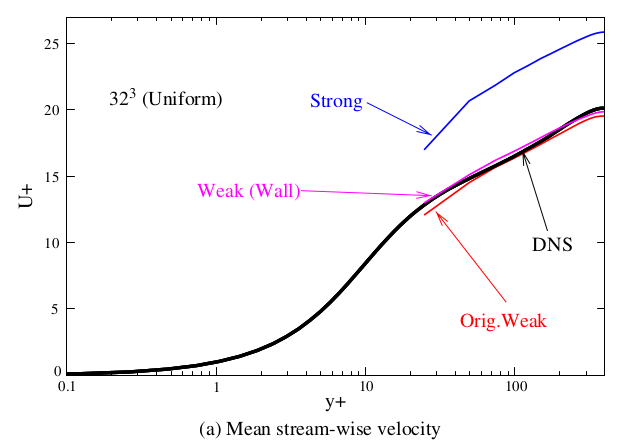
\includegraphics[width=0.98\textwidth]{figures/hughes_example.png}
	 	\end{block}
	 \end{minipage}\hfill
	 \begin{minipage}{0.49\textwidth}
	 \begin{block}{Weak Enforcement of no slip BC}
	 	\begin{align*}
	 		&a^{VMS}_{weakBC}(\vec{u}_h,p_h,\vec{v}_h,q_h):=a^{VMS}(\vec{u}_h,p_h,\vec{v}_h,q_h)\\
			-&\red{\scprb{\vec{v}_h}{2\nu \nabla^s \vec{u}_h \cdot \vec{n}}}\\
			-&\magenta{\scprb{2\nu \nabla^s \vec{v}_h \cdot \vec{n}}{\vec{u}_h-\vec{0}}}\\
			+&\blue{\scprb{\vec{v}_h \frac{C_b^I \nu}{h_b}}{\vec{u}_h-\vec{0}}}=0			
	 	\end{align*}
 	\begin{itemize}
 		\item \red{Consistency term}
 		\item \magenta{Adjoint consistency term}
 		\item \blue{Penalization of Dirichlet BC }
 	\end{itemize}
	 \end{block}
\end{minipage}

\end{frame}

\begin{frame}{Spalding Wall Law\footnote{D.B. Spalding, A single formula for the law of the wall, J. Appl. Mech. 28 (1961) 444--458}\footnote{Y. Bazilevs et al. / Comput. Methods Appl. Mech. Engrg. 196 (2007) 4853--4862}}
	\begin{minipage}{0.49\textwidth}
		\begin{block}{Weak penalty for no slip condition}
			\begin{align*}
				\scprb{\vec{v}_h \frac{C_b^I \nu}{h_b}}{\vec{u}_h-\vec{0}}
			\end{align*}
		\begin{itemize}
			\item $C_b^I=4$ user set coefficient
			\item $h_b=2\left(\vec{n}^T G\vec{n}\right)^{-1/2}$ wall-normal element mesh size
		\end{itemize}
		\end{block}
	\end{minipage}\hfill
	\begin{minipage}{0.49\textwidth}
		\begin{block}{Spalding Wall law}
			\begin{itemize}
				\item More \highlight{physical intuition}
				\item Exploiting notion of fully developed turbulence
				\item Boundary layer typically not interesting for turbulent phenomena
				\item No-slip Dirichlet BC replaced by \highlightB{traction Neumann boundary}
		\begin{equation*}
			\scprb{\vec{v}_h}{u^{*2}\frac{\vec{u}_h}{\lVert \vec{u}_h \rVert}}
		\end{equation*}
				\item $u^{*2}$ magnitude of the \highlight{wall shear stress}
				\item Consistent with the ``law of the wall''
			\end{itemize}
		\end{block}	
\end{minipage}
\end{frame}
\begin{frame}{Spalding Wall Law}
		\begin{block}{Spalding Law}
			\begin{equation*}
				\scprb{\vec{v}_h}{u^{*2}\frac{\vec{u}_h}{\lVert \vec{u}_h \rVert}}
			\end{equation*}
			\begin{itemize}
				\item Empirical relation between the mean fluid speed and the normal distance to the wall
				\item Spalding Law
				\begin{align*}
					& \blue{y^+ } \stackrel{!}{=} f(\magenta{u^+}) = \magenta{u^+} + e^{-\chi B}\left(e^{\chi \magenta{u^+}}-1-\chi \magenta{u^+}-\frac{(\chi \magenta{u^+})^2}{2} -\frac{(\chi \magenta{u^+})^3}{6}\right),\\
					&\blue{y^+ }:= \frac{y\red{u^*}}{\nu} \text{ distance from the wall in nondimensional wall units,}\\
					&\magenta{u^+}:=\frac{\lVert \vec{u}_h \rVert}{\red{u^*}} \text{ mean fluid speed in nondimensional wall units,}\\
					&\chi = 0.4,\, B =5.5.
				\end{align*}
			\end{itemize}
		\end{block}
\end{frame}

\begin{frame}{Spalding Wall Law}
	\begin{block}{Spalding Law}
		\begin{align*}
			\scprb{\vec{v}_h}{u^{*2}\frac{\vec{u}_h}{\lVert \vec{u}_h \rVert}} =&\scprb{\vec{v}_h\frac{u^{*2}}{\lVert \vec{u}_h \rVert}}{\vec{u}_h-\vec{0}} = \scprb{\vec{v}_h\red{\tau_B}}{\vec{u}_h-\vec{0}},
			&\red{\tau_B}:=\frac{u^{*2}}{\lVert \vec{u}_h \rVert}
		\end{align*}
		\begin{itemize}
			\item \highlight{$\tau_B$} makes the connection with the weak formulation where $\tau_B= \frac{C_b^I \nu}{h_b}$
			\item One extra scalar nonlinear equation to be solved ${y^+ } \stackrel{!}{=} f({u^+})$ for each boundary cell (not too expensive)
			\item Rewrite the equation in terms of $\tau_B$
			\item \highlightB{$r(\tau_B)=0$} with $r'(\tau)>0$ and  $r''(\tau)<0$ for $\tau>0$
			\item Newton's method converges if $\tau^0$ small enough (worst case bisection not too expensive)
			\item Initial guess $\tau^0= \frac{C_b^I \nu}{h_b}$ (from weak formulation)
		\end{itemize}
	\end{block}
\end{frame}

\begin{frame}{Full Order Model}
	\begin{minipage}{0.49\textwidth}
	\begin{block}{FOM}
		\begin{itemize}
			\item $\mathbb P^2-\mathbb P^2$ \highlightB{continuous Galerkin FEM} formulation
			\item Residual based Variational MultiScale discrete model 
			\item Boundary consistency terms
			\item Weak penalty for no-slip BC
			\item \highlight{Spalding Wall Law }(very fast ~1\% cost)
		\end{itemize}
	\end{block}
	\end{minipage}\hfill
	\begin{minipage}{0.49\textwidth}
\visible<2->{\begin{block}{Test: Flow Past Cylinder}
	\vspace*{-5mm}\begin{align*}
		&\mathcal{R} = [0,2.2]\times[-0.41,0.41], \mathcal{C} = \mathcal{B}([0.2,0],0.05), \\
		&D=\mathcal R \backslash \mathcal C, \qquad T_{end} = 3,\qquad \NDG= 3\cdot 122145,\\
		&u_{in} = (\mu_1,0), \quad \nu = \mu_2,\\
\only<2>{		&\text{Test 1: } Re \in [50,2.5\cdot 10^3],\\
		&\mu_1 \in [0.5,5.0],\quad  \mu_2 \in [2 \cdot 10^{-4}, 10^{-3}],\\}
\only<3>{		&\text{Test 2: }  Re \in [2.5\cdot 10^3, 2.5\cdot 10^5],\\
		&\mu_1 \in [0.5,5.0],\quad  \mu_2 \in [2 \cdot 10^{-6},2 \cdot 10^{-5}],\\}
		&\text{No slip BC on top, bottom and circle},				
	\end{align*}
\vspace*{-5mm}
\end{block}}
	\end{minipage}
\begin{center}
\only<2>{	\includemedia[
	width=0.98\linewidth,
	height=0.2\linewidth,
	activate=pageopen,
	addresource=figures/cylinder_weak.avi,
	flashvars={source=figures/cylinder_weak.avi
			&loop=true 
			&autoPlay=true }
	]{}{VPlayer.swf}}
\only<3>{	\includemedia[
width=0.98\linewidth,
height=0.2\linewidth,
activate=pageopen,
addresource=figures/cylinder_turb_weak.avi,
flashvars={source=figures/cylinder_turb_weak.avi
	&loop=true 
	&autoPlay=true }
]{}{VPlayer.swf}}
\end{center}
\end{frame}

\section{Reduced Order Model: Galerkin Projection}
\begin{frame}{Reduced Order Model\footnote{Stabile, Giovanni, et al. "A reduced order variational multiscale approach for turbulent flows." Advances in Computational Mathematics 45 (2019): 2349-2368.}}
	\begin{minipage}{0.49\textwidth}
		\begin{block}{Solution Manifold Compression}
			\begin{itemize}
			\item Proper Orthogonal Decomposition (\highlightB{POD})
			\item Collection of \highlightB{snapshots} $\lbrace [u_h,p_h,\tau_{B,h}](t^{i_0},\mu_1^{i_1},\mu_2^{i_2}) \rbrace_{i\in \mathcal{T}} \in \VDG$
			\item Generation of \highlightB{$\VRB$} component by component
			\item No need of supremizer$^5$
			\end{itemize}
		\end{block}
	\visible<3->{
\begin{block}{Spalding coefficient reconstruction}
	\begin{itemize}
		\item For $\tau_{B,h}$ POD-Galerkin and then Newton
		\item Problem: \highlightB{Newton does not converge} for reduced $\tau_{B,RB}$ equation
		\item Multi-layer perceptron NN $u_{RB} \to \tau_{B,RB}$?
	\end{itemize}
\end{block}	
}
	\end{minipage}\hfill
\begin{minipage}{0.49\textwidth}
\visible<2->{	\begin{block}{Reconstruction}
		\begin{itemize}
		\item \highlightB{POD-Galerkin}
			\begin{itemize}
				\item $F(u_h)=0\Longrightarrow \VRB^T F(\VRB u_{RB})=0$
				\item Less equations
				\item \highlight{Hyper-reduction} needed to decrease costs (not today)
				\item \highlightB{Physics} based
				\item Less nonlinear iterations
				\item For the moment no computational advantage
			\end{itemize}
		\item \highlight{POD-NN}
		\begin{itemize}
			\item NN learn map $u_{RB}(t,\mu_1,\mu_2)$ from training set
			\item Very \highlight{fast} reconstruction
			\item \highlightB{No physics} involved
			\item Needs \highlightB{many snapshots} for different parameters (too expensive offline phase)
		\end{itemize}
		\end{itemize}
	\end{block}
}
\end{minipage}
\end{frame}

\begin{frame}{POD results: \highlightB{Test1}, 20 parameters, 150 timesteps}
	\begin{tabular}{ccc}
		$u$&$p$&$\tau$\\
		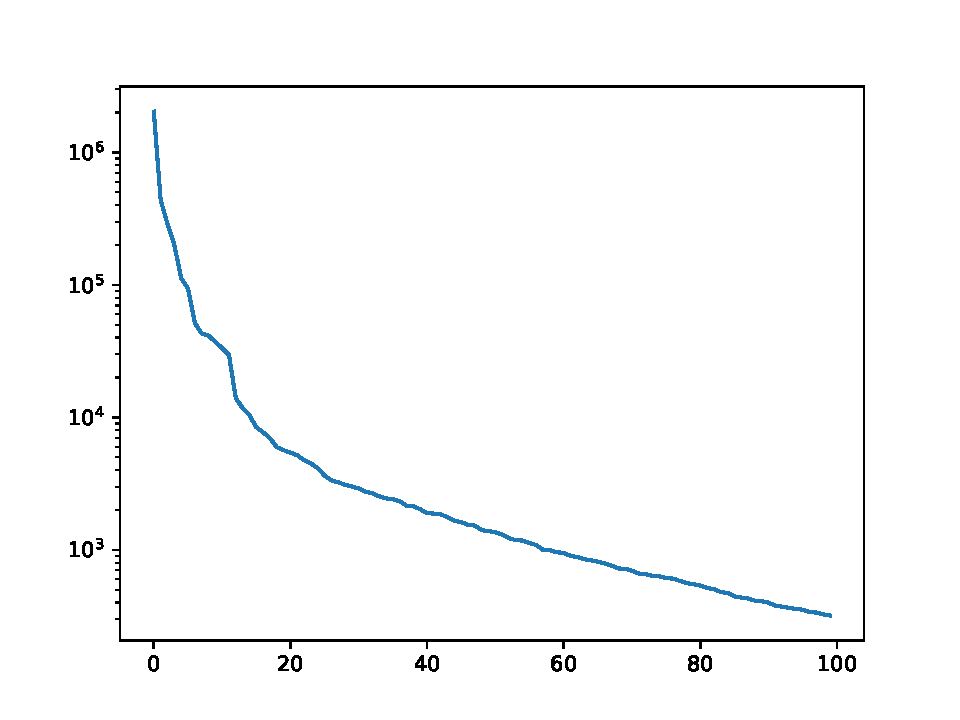
\includegraphics[width=0.31\textwidth]{figures/cylinder_weak_eigs_u.pdf}&
		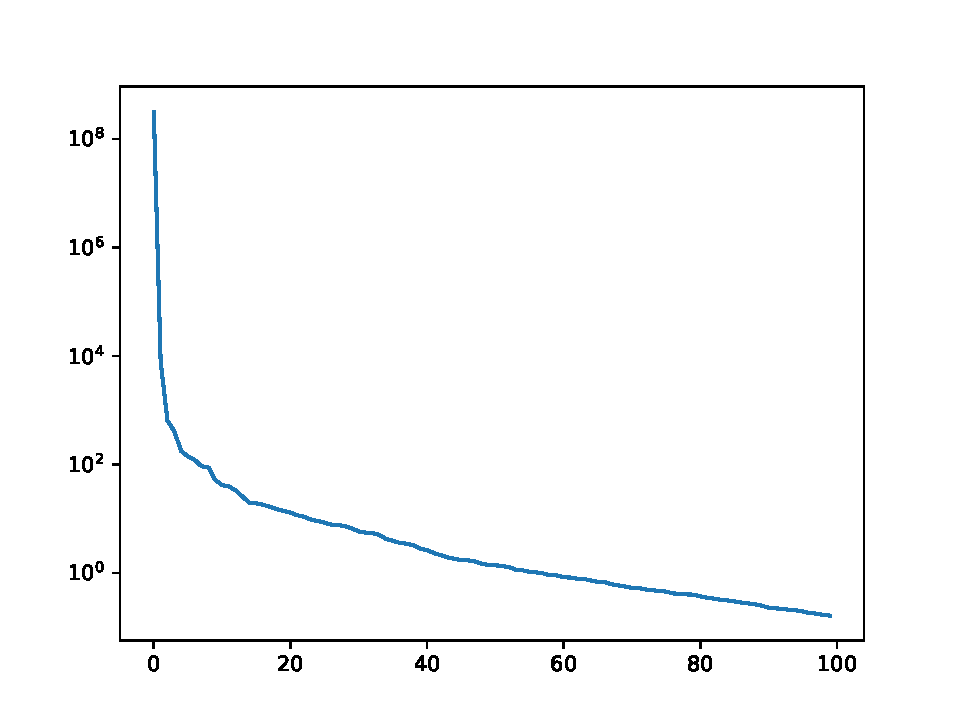
\includegraphics[width=0.31\textwidth]{figures/cylinder_weak_eigs_p.pdf}&
		$\Leftarrow$ Weak BC, Spalding BC $\Downarrow$
		\\
		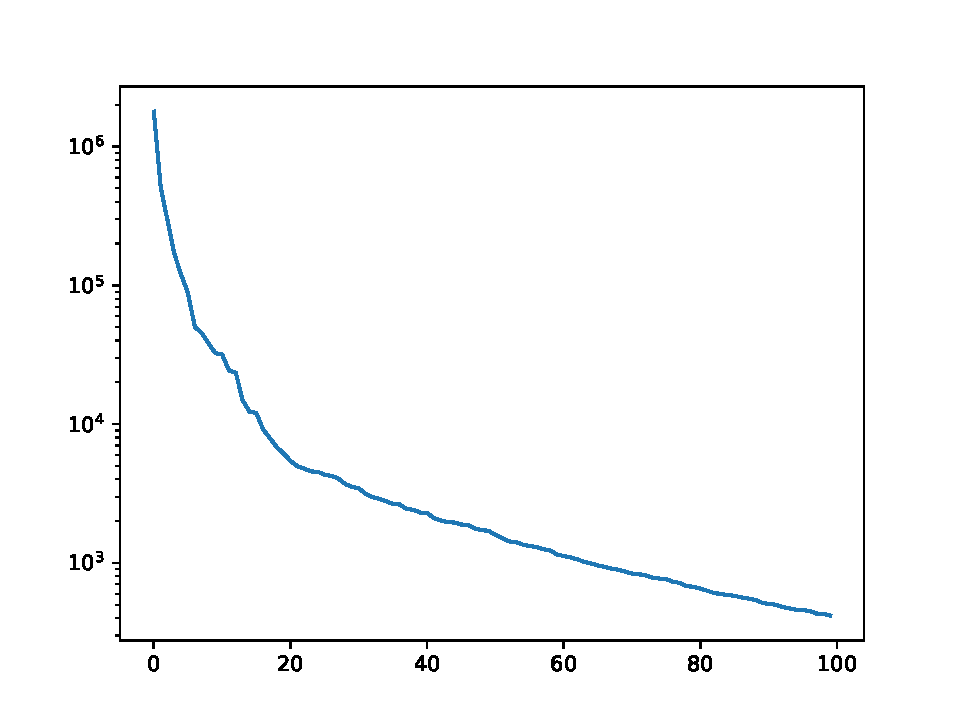
\includegraphics[width=0.31\textwidth]{figures/cylinder_spalding_eigs_u.pdf}&
		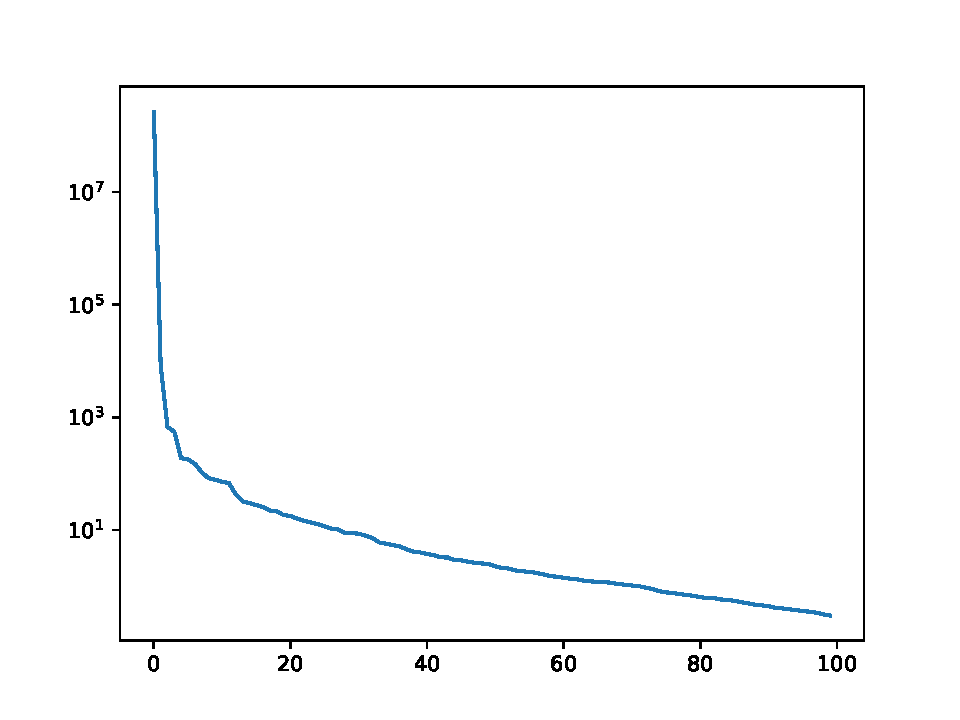
\includegraphics[width=0.31\textwidth]{figures/cylinder_spalding_eigs_p.pdf}&
		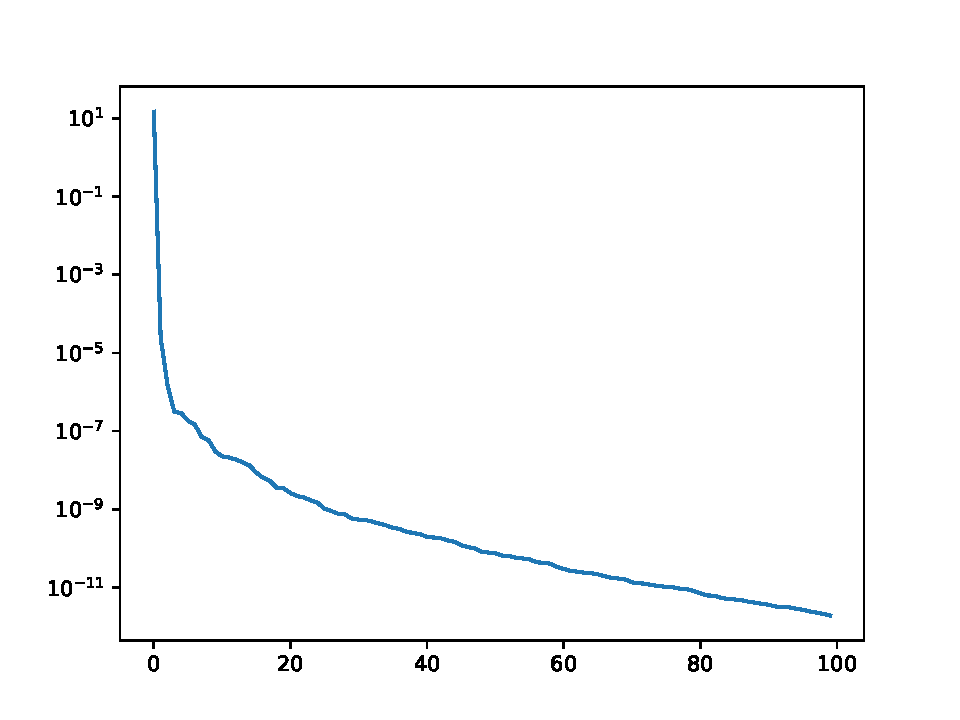
\includegraphics[width=0.31\textwidth]{figures/cylinder_spalding_eigs_tau.pdf}
	\end{tabular}\hfill
\end{frame}

\begin{frame}{POD results: \highlightB{Test2}, 20 parameters, 150 timesteps}
	\begin{tabular}{ccc}
		$u$&$p$&$\tau$\\
		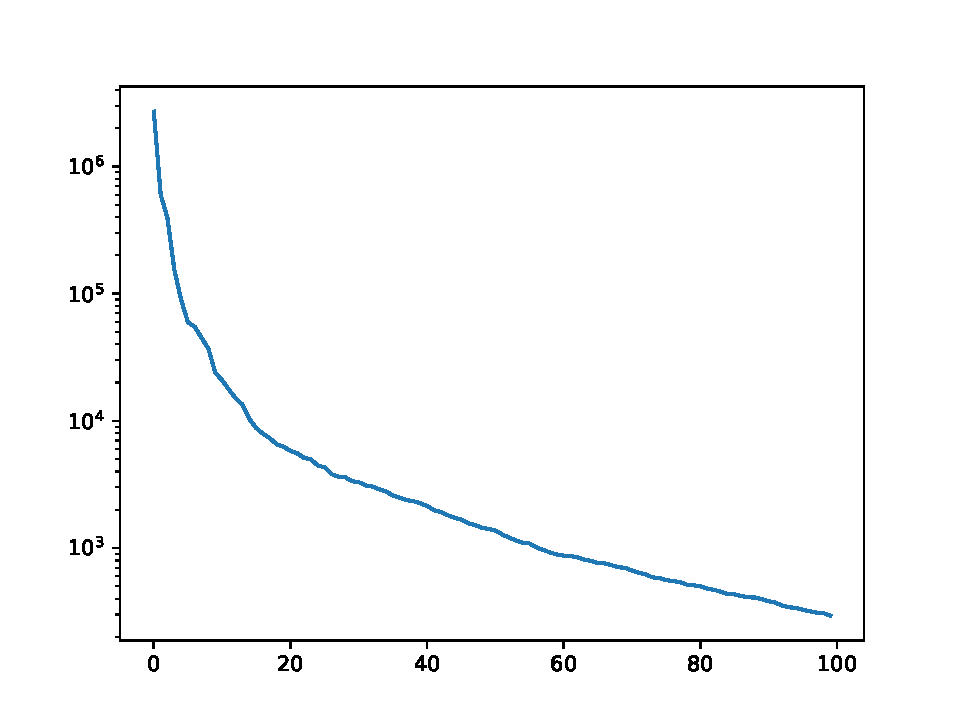
\includegraphics[width=0.31\textwidth]{figures/cylinder_turb_weak_eigs_u.pdf}&
		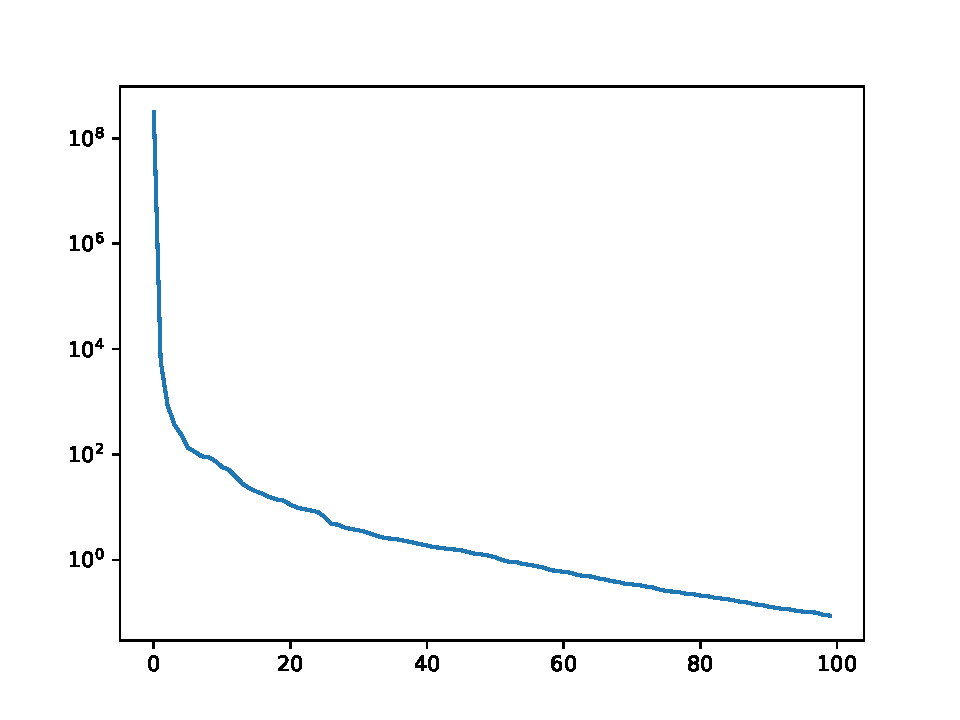
\includegraphics[width=0.31\textwidth]{figures/cylinder_turb_weak_eigs_p.pdf}&
		$\Leftarrow$ Weak BC, Spalding BC $\Downarrow$
		\\
		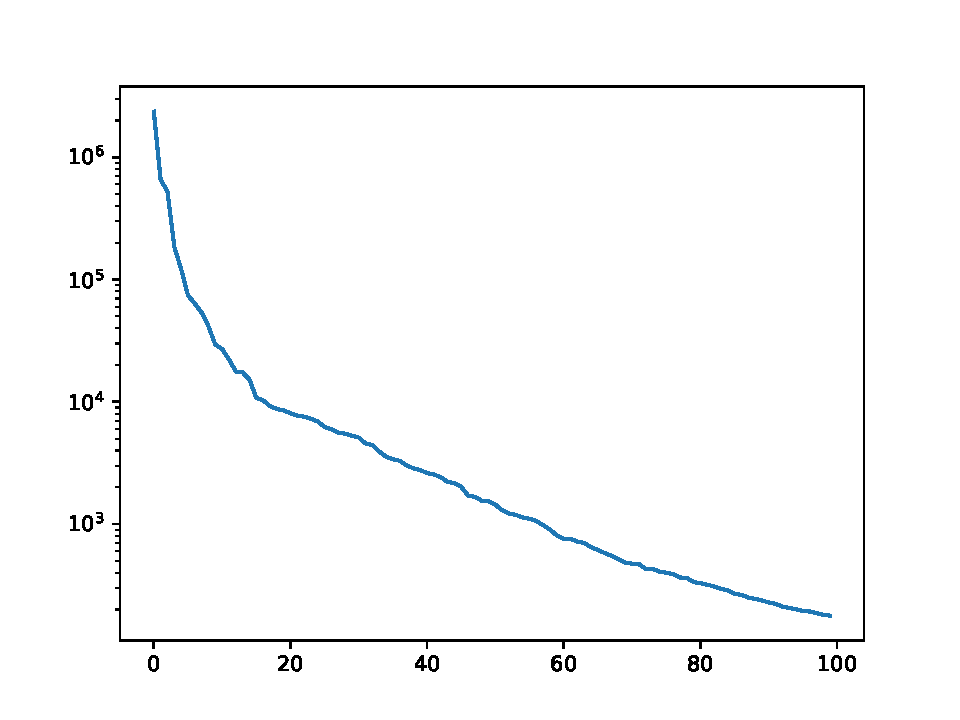
\includegraphics[width=0.31\textwidth]{figures/cylinder_turb_spalding_eigs_u.pdf}&
		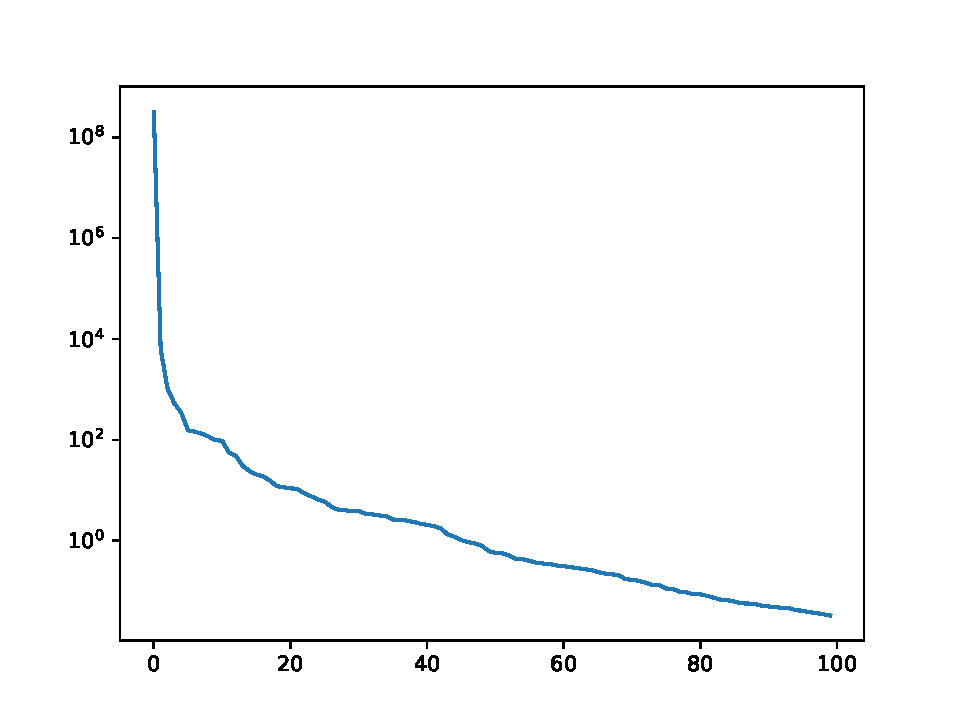
\includegraphics[width=0.31\textwidth]{figures/cylinder_turb_spalding_eigs_p.pdf}&
		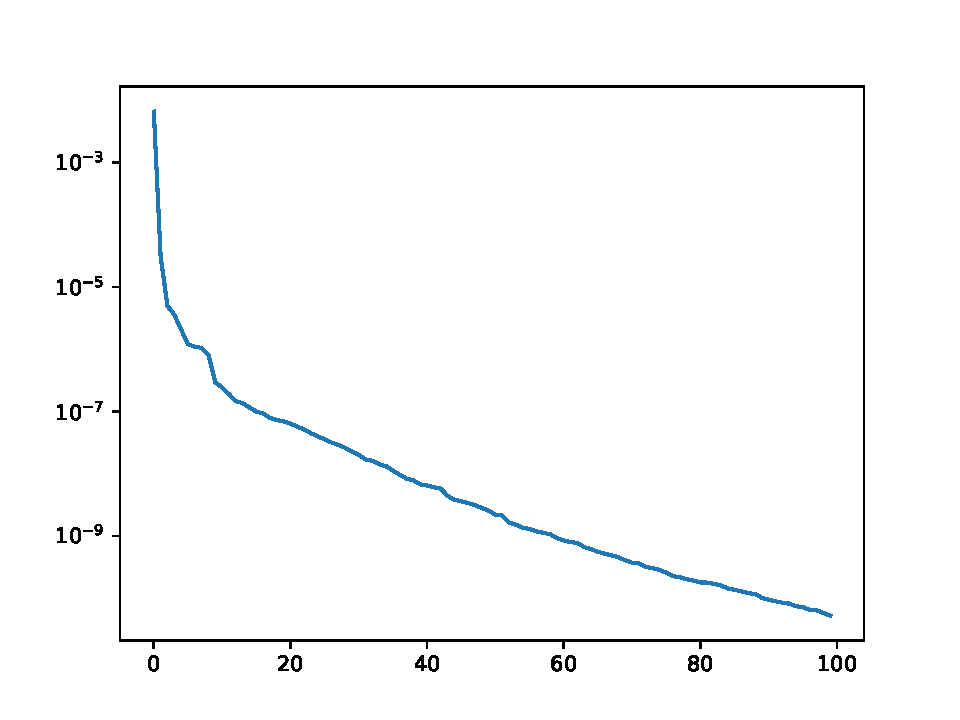
\includegraphics[width=0.31\textwidth]{figures/cylinder_turb_spalding_eigs_tau.pdf}
	\end{tabular}\hfill
\end{frame}

\begin{frame}{\highlight{POD projection} error: \highlightB{Test1},  $(u_{in},\nu)=(1,0.001)$}
	
	\begin{center}
		$N_{POD}^u=N_{POD}^p=100$, $N_{POD}^\tau=30$
	\begin{tabular}{cc}
		Weak BC& Spalding\\
		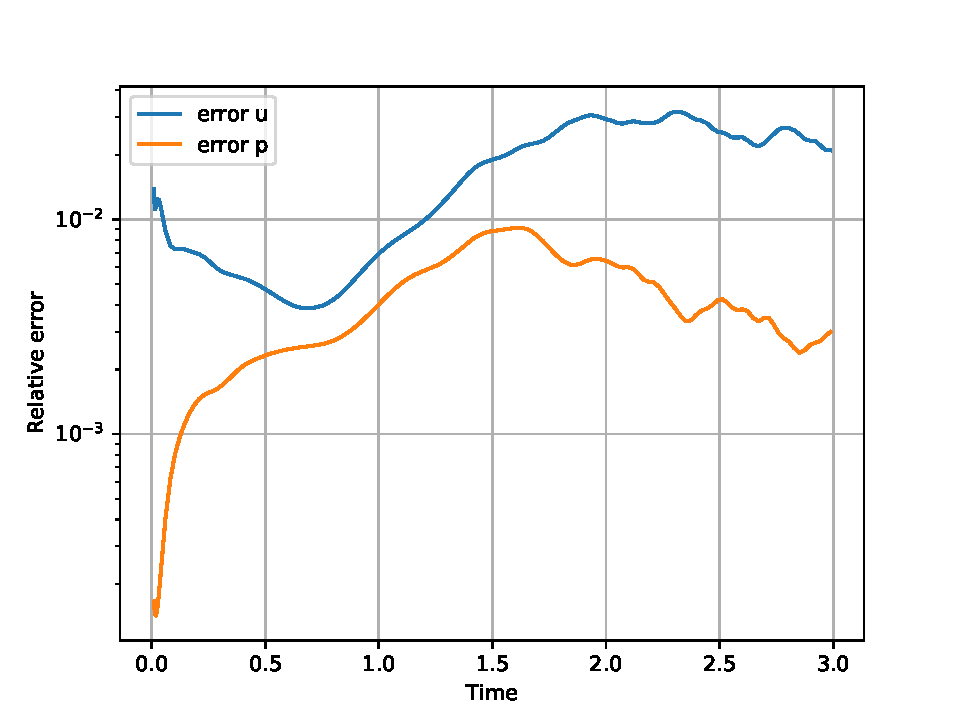
\includegraphics[width=0.49\textwidth]{figures/cylinder_weak_errors_vs_time_proj.pdf}&
		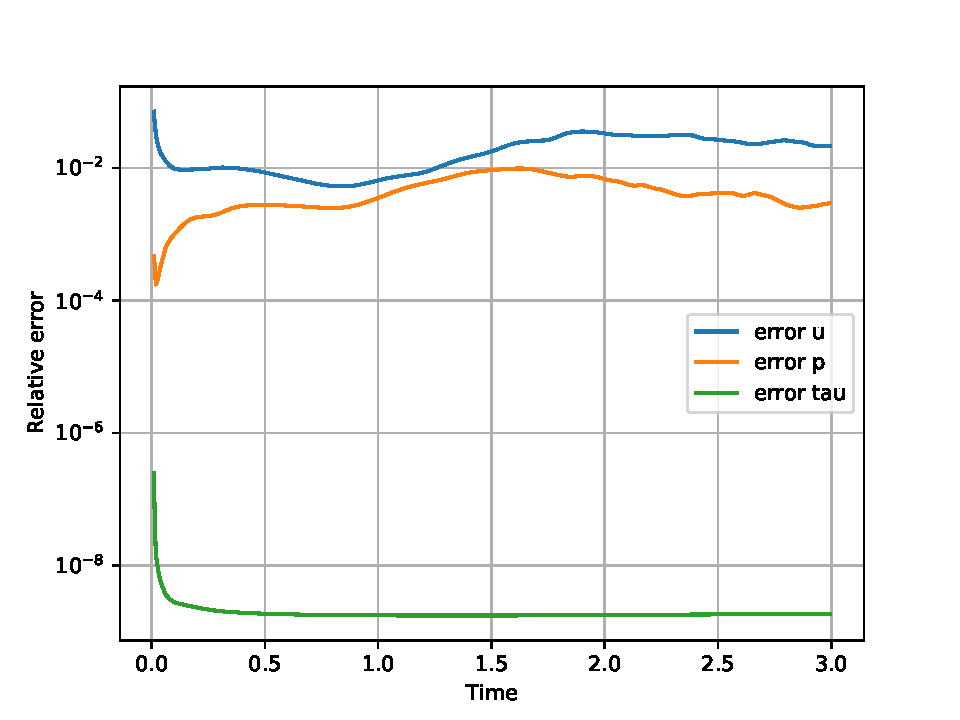
\includegraphics[width=0.49\textwidth]{figures/cylinder_spalding_errors_vs_time_proj.pdf}
	\end{tabular}
	\end{center}
\end{frame}


\begin{frame}{\highlight{POD projection }error: \highlightB{Test2}, $(u_{in},\nu)=(1,2\cdot 10^{-6})$}
	\begin{center}
		$N_{POD}^u=N_{POD}^p=100$, $N_{POD}^\tau=30$
		\begin{tabular}{cc}
			Weak BC& Spalding\\
			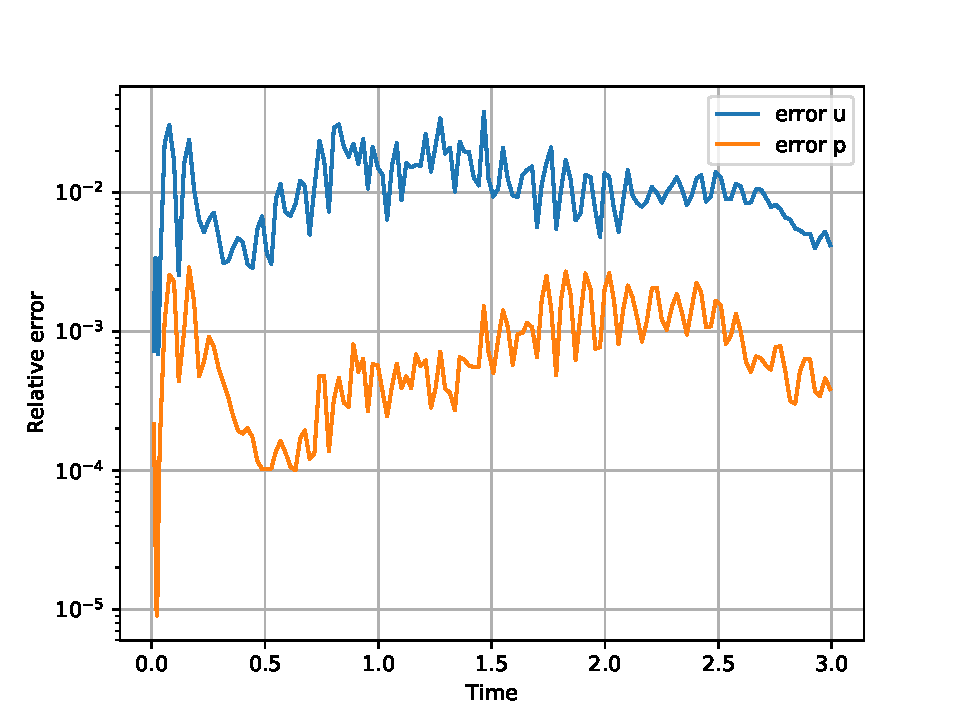
\includegraphics[width=0.49\textwidth]{figures/cylinder_turb_weak_errors_vs_time_proj.pdf}&
			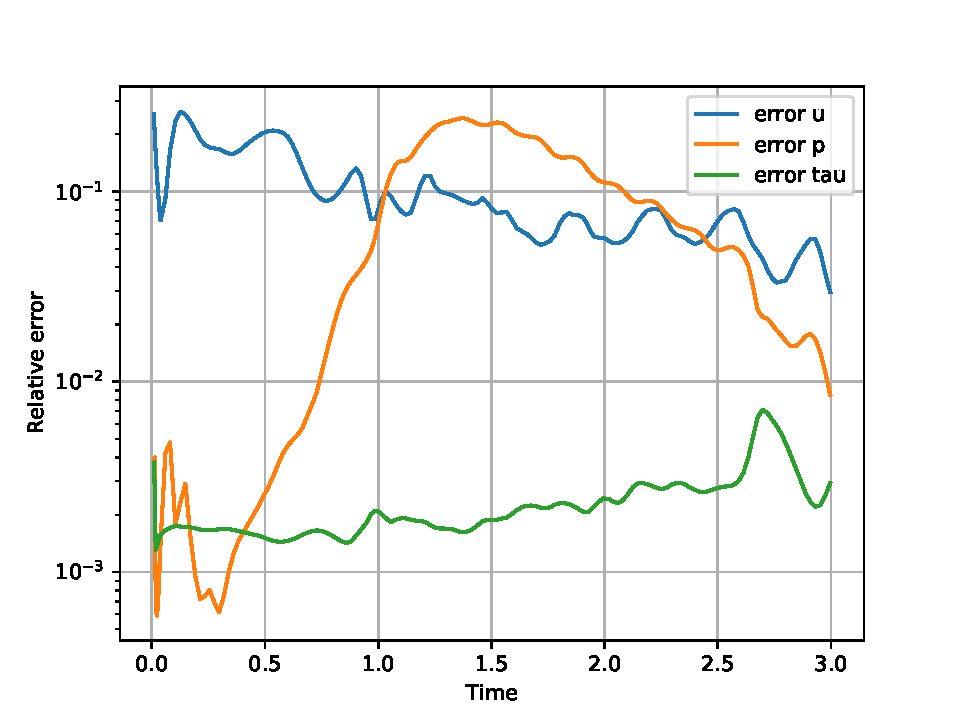
\includegraphics[width=0.49\textwidth]{figures/cylinder_turb_spalding_errors_vs_time_proj.pdf}
		\end{tabular}
	\end{center}
\end{frame}

\begin{frame}{\highlight{POD-Galerkin} error: \highlightB{Test1}, $(u_{in},\nu)=(1,0.001)$}
	\begin{center}
		$N_{POD}^u=N_{POD}^p=100$, $\tau$ exact
		\begin{tabular}{cc}
			Weak BC& Spalding\\
			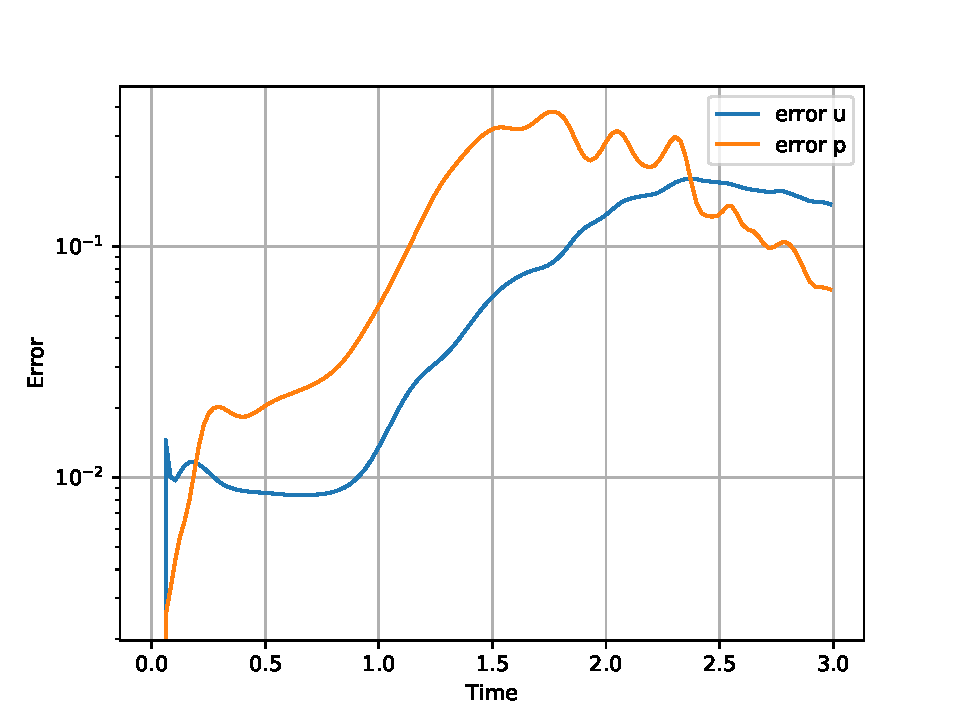
\includegraphics[width=0.49\textwidth]{figures/cylinder_weak_errors_RB_vs_time.pdf}&
			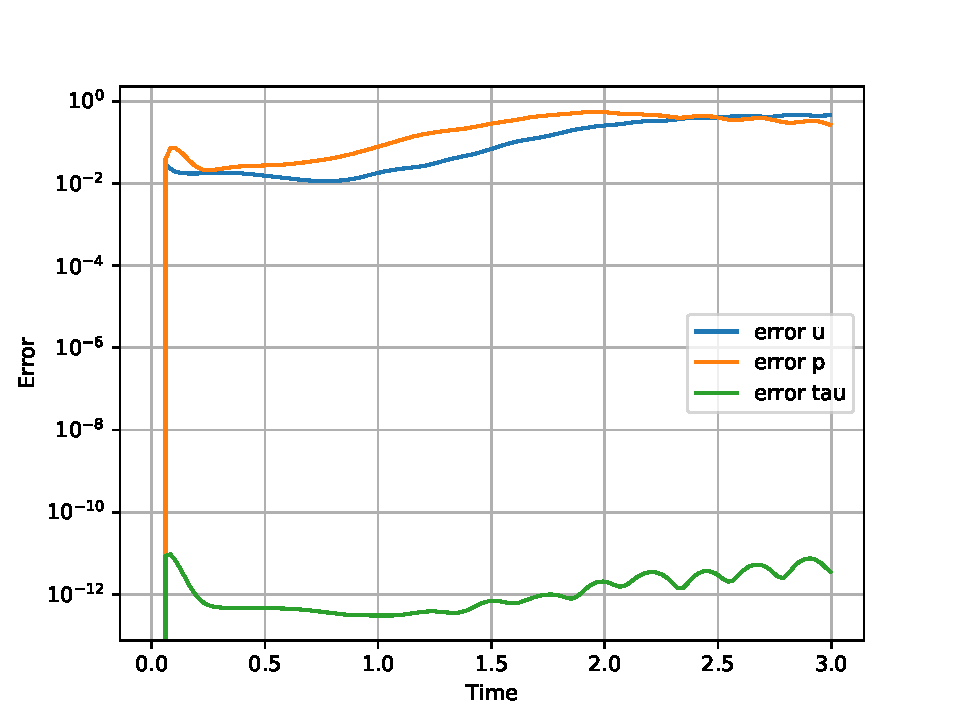
\includegraphics[width=0.49\textwidth]{figures/cylinder_spalding_errors_RB_vs_time.pdf}
		\end{tabular}
	\end{center}
\end{frame}


\begin{frame}{\highlight{POD-Galerkin} error: \highlightB{Test2}, $(u_{in},\nu)=(1,2\cdot 10^{-6})$}
	\begin{center}
		$N_{POD}^u=N_{POD}^p=100$, $\tau$ exact
		\begin{tabular}{cc}
			Weak BC& Spalding\\
			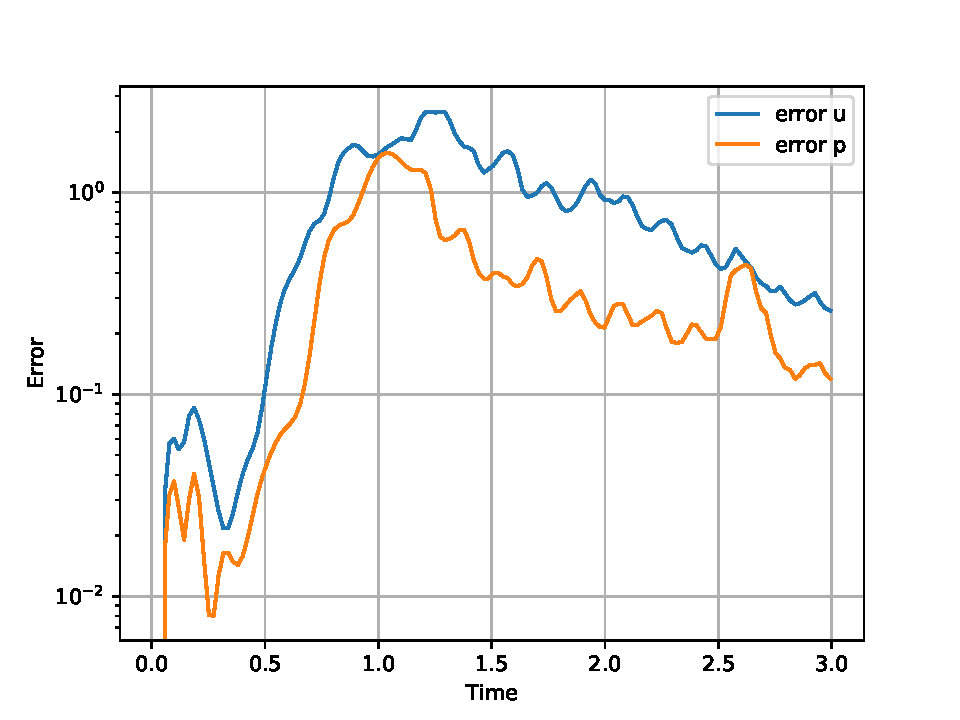
\includegraphics[width=0.49\textwidth]{figures/cylinder_turb_weak_errors_RB_vs_time.pdf}&
			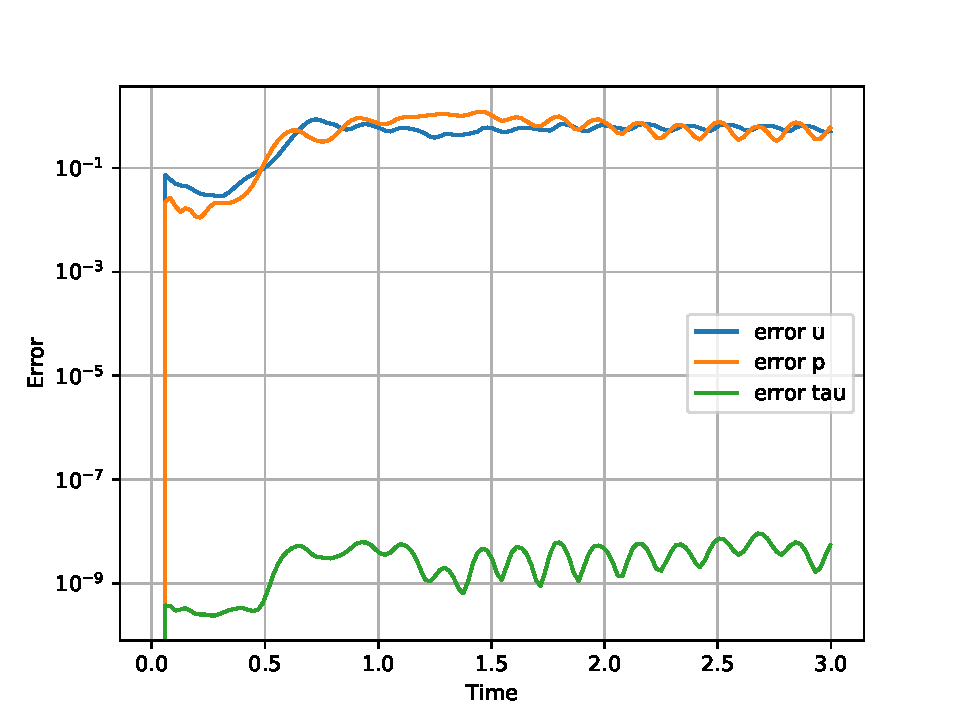
\includegraphics[width=0.49\textwidth]{figures/cylinder_turb_spalding_errors_RB_vs_time.pdf}
		\end{tabular}
	\end{center}
\end{frame}




\begin{frame}{\highlightB{Test1} \highlight{Weak} BC: POD-Galerkin (top) vs FOM (bottom)}
	\includemedia[
		width=0.98\linewidth,
		height=0.8\textheight,
		activate=pageopen,
		addresource=figures/cylinder_weak_uROMvsFOM.avi,
		flashvars={source=figures/cylinder_weak_uROMvsFOM.avi
			&loop=true 
			&autoPlay=true }
		]{}{VPlayer.swf}
\end{frame}

\begin{frame}{\highlightB{Test1} \highlight{Spalding} BC: POD-Galerkin (top) vs FOM (bottom)}
	\includemedia[
	width=0.98\linewidth,
	height=0.8\textheight,
	activate=pageopen,
	addresource=figures/cylinder_spalding_uROMvsFOM.avi,
	flashvars={source=figures/cylinder_spalding_uROMvsFOM.avi
		&loop=true 
		&autoPlay=true }
	]{}{VPlayer.swf}
\end{frame}


\begin{frame}{\highlightB{Test2} \highlight{Weak} BC: POD-Galerkin (top) vs FOM (bottom)}
	\includemedia[
	width=0.98\linewidth,
	height=0.8\textheight,
	activate=pageopen,
	addresource=figures/cylinder_turb_weak_uFOMvsRB.avi,
	flashvars={source=figures/cylinder_turb_weak_uFOMvsRB.avi
		&loop=true 
		&autoPlay=true }
	]{}{VPlayer.swf}
\end{frame}

\begin{frame}{\highlightB{Test2} \highlight{Spalding} BC: POD-Galerkin (top) vs FOM (bottom)}
	\includemedia[
	width=0.98\linewidth,
	height=0.8\textheight,
	activate=pageopen,
	addresource=figures/cylinder_turb_spalding_uRBvsFOM.avi,
	flashvars={source=figures/cylinder_turb_spalding_uRBvsFOM.avi
		&loop=true 
		&autoPlay=true }
	]{}{VPlayer.swf}
\end{frame}

\begin{frame}{Comments on POD-Galerkin}
\only<1-3,5>{	\begin{minipage}{0.49\textwidth}
	\begin{block}{Vortex shedding start}
		\begin{itemize}
			\item The \highlight{vortex shedding} in FOM is dictated purely by the (triangular) mesh
			\item No reasons why also in ROM it should start at the same time and in the same direction
			\item Starting the ROM simulation after vortex shedding (at time $t=1$)
		\end{itemize}
	\end{block}
	\end{minipage}}
	\hfill\begin{minipage}{0.47\textwidth}
\only<5->{
\begin{block}{Weak BC vs Spalding}
	\begin{itemize}
		\item Spalding has larger error in representation
		\item Spalding has little worse behavior in POD-Galerkin
		\item In past simulations, $\tau_B$ computed as FOM ($\approx 250$ DOFs)
	\end{itemize}
\end{block}}
\only<2>{
	\begin{center}
	\Large Weak BC Test2 ROM from $t=0$
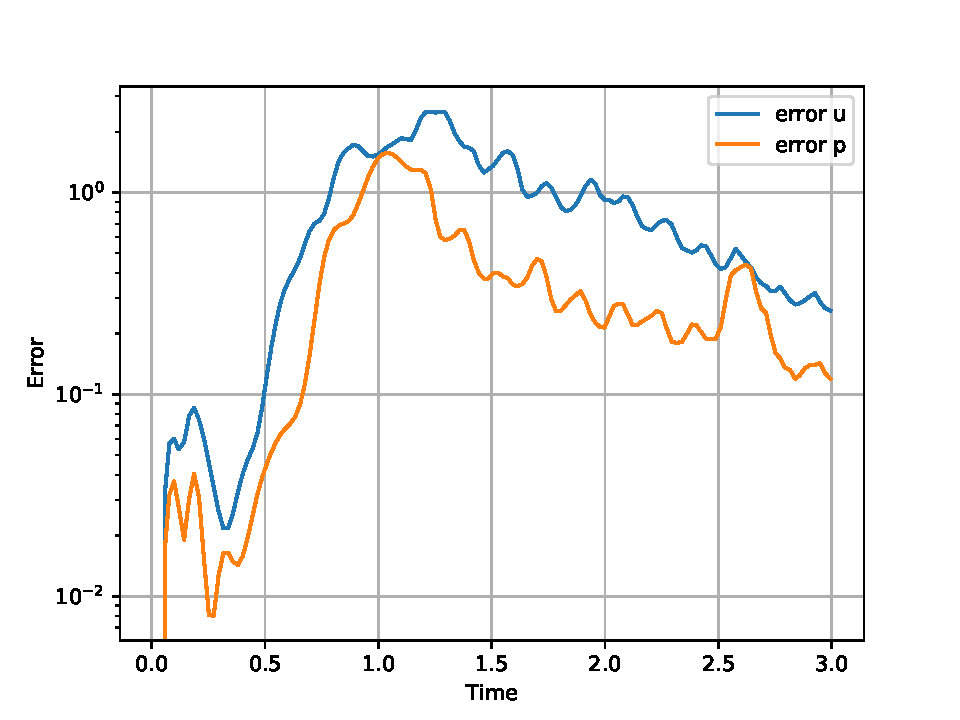
\includegraphics[width=0.99\textwidth]{figures/cylinder_turb_weak_errors_RB_vs_time.pdf}
	\end{center}
}
\only<3>{
	\begin{center}
		\Large Weak BC Test2 ROM from $t=1$
		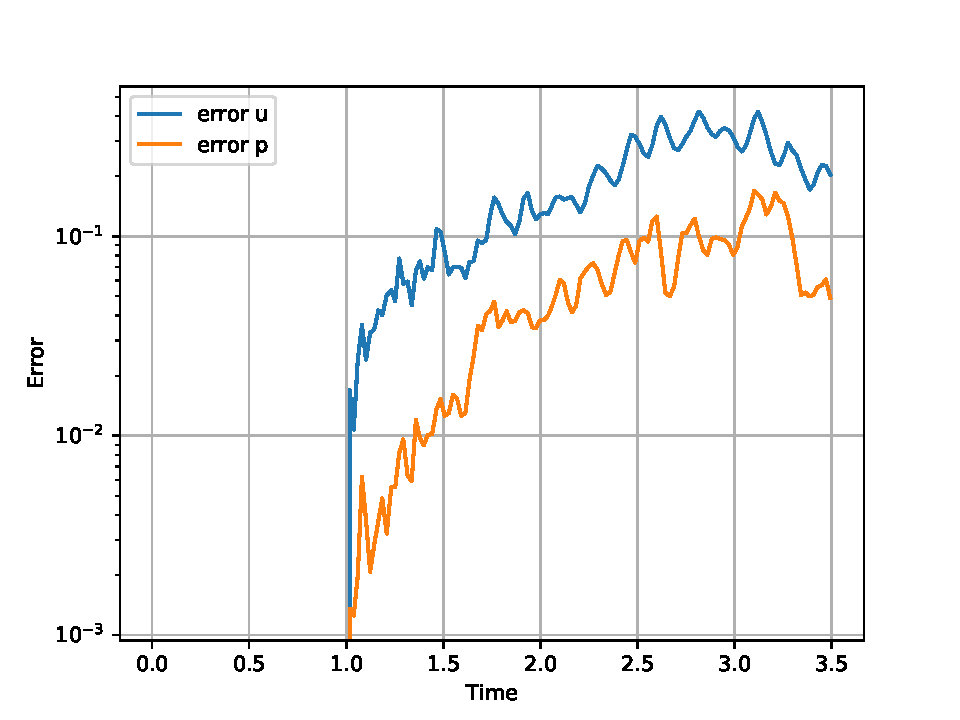
\includegraphics[width=0.99\textwidth]{figures/cylinder_turb_weak_later_errors_RB_vs_time.pdf}
	\end{center}
}
\end{minipage}
\only<4>{\begin{center} \vspace*{-8mm}
	\Large Weak BC Test2 ROM from $t=1$
		\includemedia[
	width=0.98\linewidth,
	height=0.8\textheight,
	activate=pageopen,
	addresource=figures/cylinder_turb_weak_uFOMvsRB_later.avi,
	flashvars={source=figures/cylinder_turb_weak_uFOMvsRB_later.avi
		&loop=true 
		&autoPlay=true }
	]{}{VPlayer.swf}
		\end{center}
}
%
%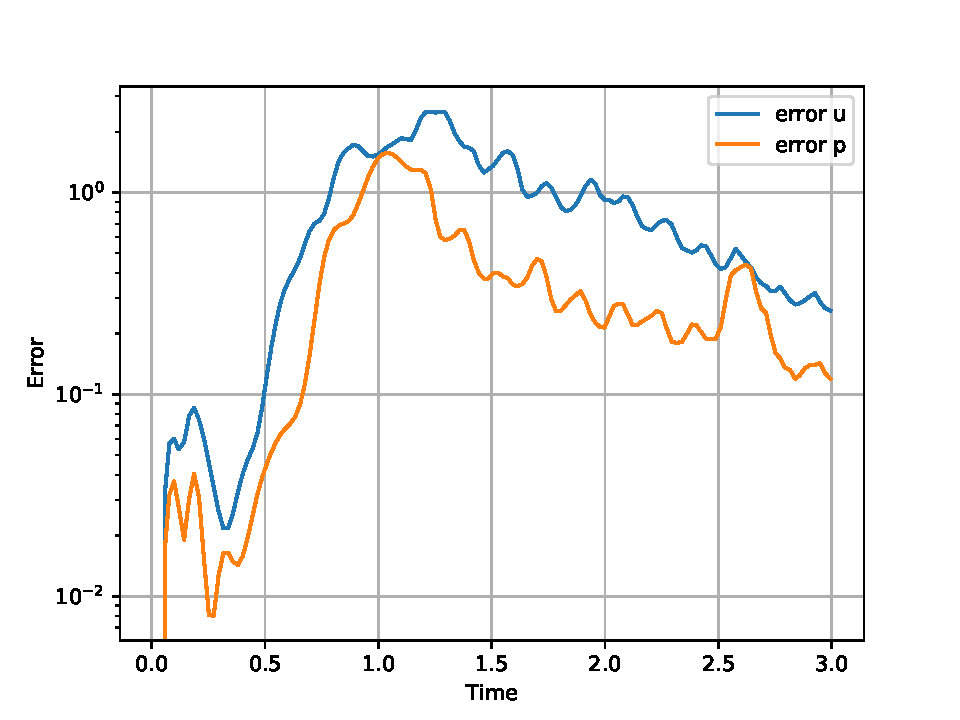
\includegraphics[width=0.31\textwidth]{figures/cylinder_turb_weak_errors_RB_vs_time.pdf}
%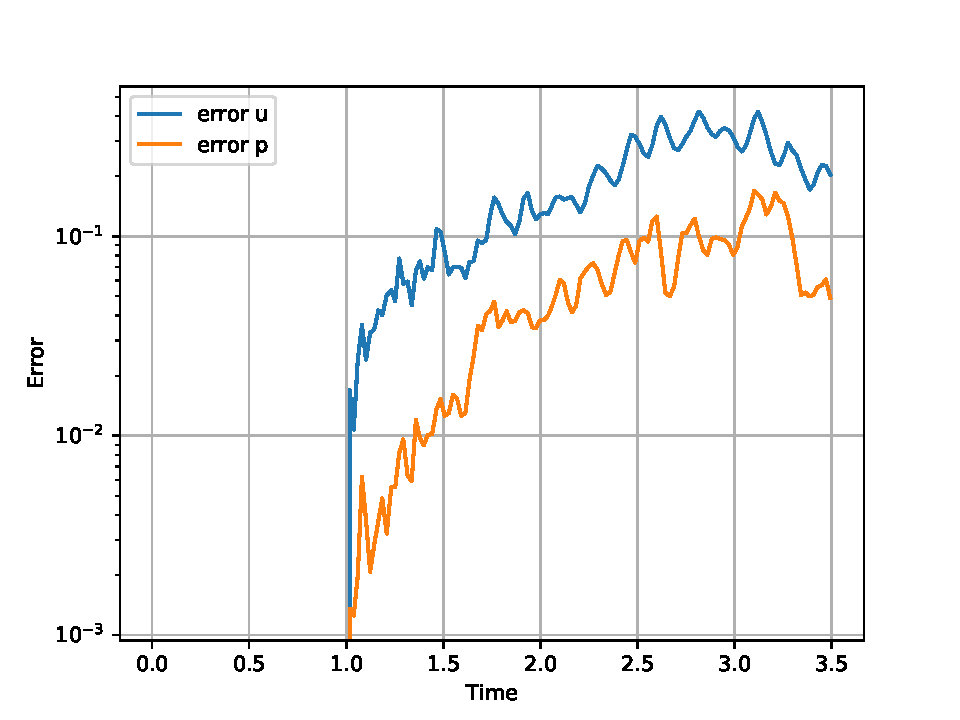
\includegraphics[width=0.31\textwidth]{figures/cylinder_turb_weak_later_errors_RB_vs_time.pdf}
\end{frame}

\begin{frame}{POD-NN}
	\begin{minipage}{0.49\textwidth}
		\begin{block}{POD-NN}
			\begin{itemize}
				\item Training set as POD: 20 params, 150 timesteps (3000 snapshots)
				\item Goal: learn map $(t,\mu_0,\mu_1)\to u_{RB}$
				\item NN setting 
				\begin{itemize}
					\item multi-layer perceptron 
					\item 4 hidden nodes 
					\item 100 neurons each
					\item Various activation functions
				\end{itemize}
				\item For $u$ and $p$ the loss struggle at decaying
				\item For $\tau$ already better results, but dangerous to be used alone (time consistency)
			\end{itemize}
		\end{block}
	\end{minipage}\hfill
	\begin{minipage}{0.49\textwidth}
	\begin{block}{Prediction of $\tau$}
		It might be safer to predict $\tau_B(u)$
		\begin{itemize}
			\item Learn $u_{RB}\to \tau_{B,RB}$
			\item NN as before
			\item Errors $\approx 6\%$ on a test set
			\item Not really helpful in reducing the computational costs (solving for $\tau_B$ already cheap (1\% of all costs)
			\item Still not physics based
		\end{itemize}
	\end{block}
\end{minipage}
\end{frame}


\section{Conclusions}

\begin{frame}[c]{Summary and perspectives\footnote{N. Ahmed, T. C. Rebollo, V. John and S. Rubino. Analysis of a Full Space–Time Discretization of the Navier–Stokes Equations by a Local Projection Stabilization Method. IMA Journal of Numerical Analysis, Vol. 37, pp. 1437–1467, 2017.}}
	\begin{minipage}[t]{0.49\textwidth}
		\begin{beamercolorbox}[sep=0.5em,wd=\textwidth]{blockcolor1}
				\centering
			\highlight{\LARGE Summary}
		\end{beamercolorbox}
		\begin{beamercolorbox}[sep=0.5em,wd=\textwidth]{blockcolor1}
			\Large
			\begin{itemize}
				\item LES-VMS model for Navier-Stokes in FEM
				\item Weak Boundary Conditions
				\item Spalding Law
				\item POD-Galerkin
				\item POD-NN (just started)
			\end{itemize}
				
		\end{beamercolorbox}
	\end{minipage}
	\begin{minipage}[t]{0.49\textwidth}
	\begin{beamercolorbox}[sep=0.5em,wd=\textwidth]{blockcolor1}
		\centering
		\highlight{\LARGE Perspectives}
	\end{beamercolorbox}
	\begin{beamercolorbox}[sep=0.5em,wd=\textwidth]{blockcolor1}
		\Large
		\begin{itemize}
			\item Hyper-reduction (EIM or overcollocation)
			\item Extend to other models with Local Projection Stabilization (LPS) onto sub-filter scale$^6$
			\item 3D turbulent simulations
			\item Improve the architecture for POD-NN to have a comparison with POD-Galerkin
		\end{itemize}
		
	\end{beamercolorbox}
\end{minipage}

\end{frame}

\begin{frame}[c]
\begin{beamercolorbox}[sep=1em,wd=\textwidth]{blockcolor1}
		\centering {\large \highlight{Literature}}\\
\begin{itemize}
	\item Y. Bazilevs, T.J.R. Hughes. "Weak imposition of Dirichlet boundary conditions
	in fluid mechanics." Computers \& Fluids 36 (2007) 12--26.
	\item Y. Bazilevs, C. Michler, V.M. Calo, T.J.R. Hughes. "Weak Dirichlet boundary conditions for wall-bounded turbulent flows." Comput. Methods Appl. Mech. Engrg. 196 (2007) 4853--4862.
	\item D.B. Spalding, A single formula for the law of the wall, J. Appl. Mech. 28 (1961) 444--458.
	\item Stabile, Giovanni, et al. "A reduced order variational multiscale approach for turbulent flows." Advances in Computational Mathematics 45 (2019): 2349-2368.
	\item N. Ahmed, T. C. Rebollo, V. John and S. Rubino. Analysis of a Full Space–Time Discretization of the Navier–Stokes Equations by a Local Projection Stabilization Method. IMA Journal of Numerical Analysis, Vol. 37, pp. 1437–1467, 2017.
	
\end{itemize}
	\end{beamercolorbox}
\pause\begin{beamercolorbox}[sep=1em,wd=\textwidth]{blockcolor1}
	\centering \LARGE \highlightB{THANK YOU!}
\end{beamercolorbox}
\end{frame}






\end{document}
